\section{Tracks}\label{Tracks}
In the TORCS environment is it possible to change the tracks the car is driving in. This is done, to see how different tracks will affect the training. The different tracks are also used for testing. It is possible to test if the car has learned how to drive, by training the car on one track, and then testing it on another track. The car should then be able to drive on both tracks. This is also known from supervised learning, where a network is trained on one set of data, and tested on another set of data to see how the network performs.   

The setup for testing is described in the introduction to this \Cref{cha:Result}. The same setup is then used on all the different tracks the car has been trained on, this is done to make sure that the results from the different tracks have the same parameters.  

In the TORCS environment, there is a wide selection of different tracks. For getting the agent to learn how to drive, a simple track was decided. This was done due to more complicated tracks, had more obstacles like bridges, trees, and mountains. A problem with these obstacles is if the agent should turn left for the first time and it sees many trees at the turning point. Then the agent could end up learning it should turn left every time it sees a tree. It will take longer time for the agent to learn how to drive if there are many obstacles on the track.   

Another issue seen on more complicated tracks is the road on the track. This road can sometimes change the same track. The edges of the road can also change on the same track. The changes of the road and edges will make it complicated for an agent to learn something, and maybe end up not learning how to drive. Another problem is it will also increase the training time. 

The track shouldn't be too simple, it still must look like a real road, it needs to have some turns both left and right, so it learns how to drive. 

The track mostly used in this project is a simple track, which has the same road type in the whole track. The track doesn't have obstacles, only grass around the road, and the edges of the road is red and white stripes on the whole track. The track has both left and right turns, and places with no turning. It is then possible for the agent to learn different scenarios. The track mostly used in this project can be seen on \Cref{fig:track_simple_1}.

\begin{figure}[H]
	\centering
	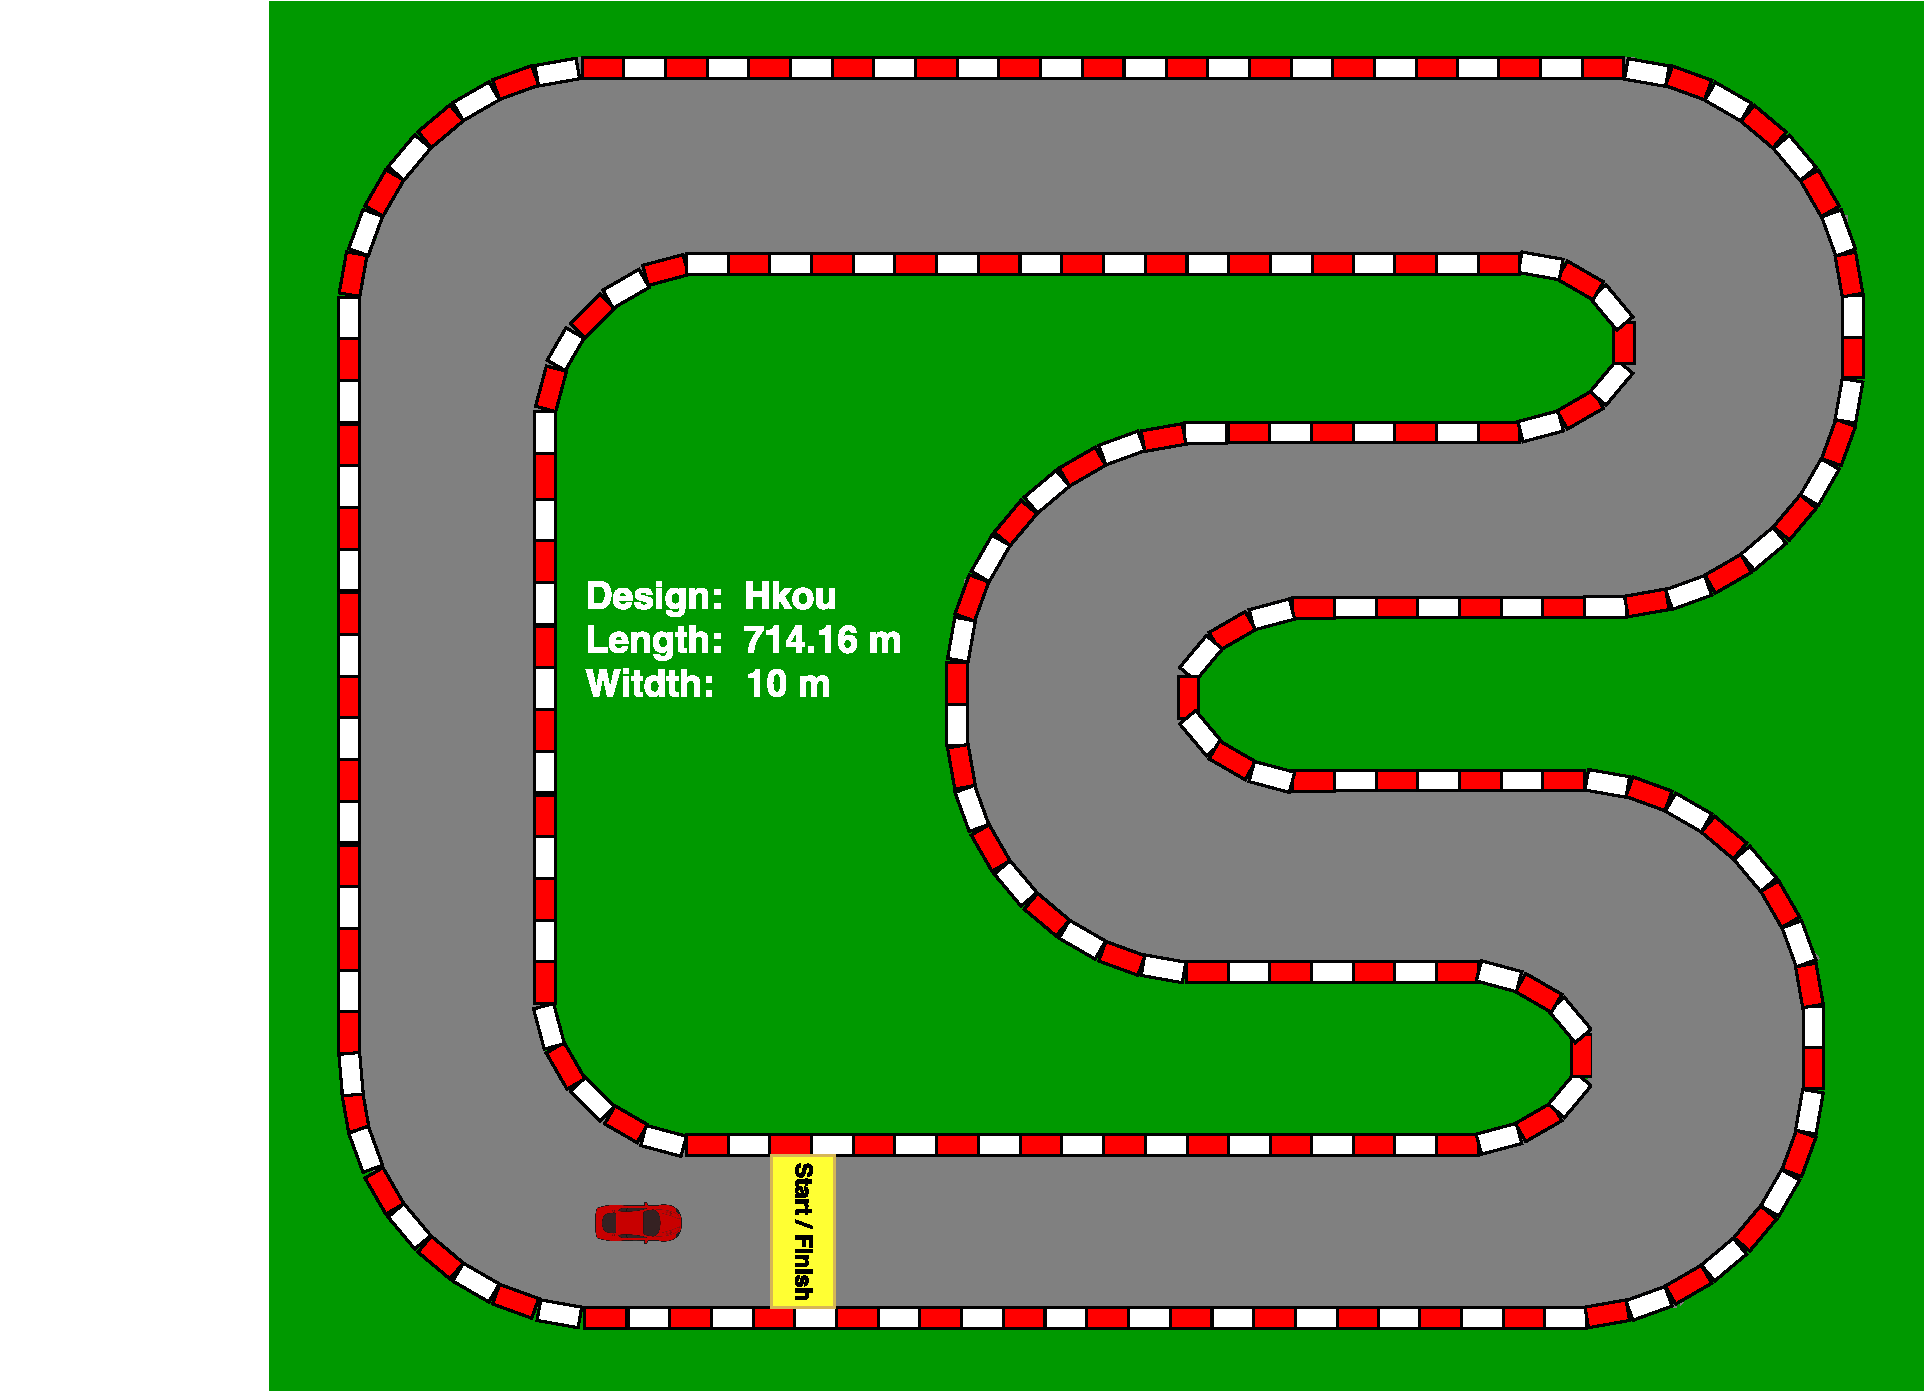
\includegraphics[width=1\textwidth]{Figures/Result/track_simple_1.pdf}
	\caption{The first track used is called $simple\_1$ made by Hkou}
	\label{fig:track_simple_1}
\end{figure}

To find different tracks, to train and test the agent on, it has to look similar to the one on \Cref{fig:track_simple_1}. It is because the agent only learns from the input image. If it should be possible to test the trained agent, it should see some of the same things on the test track as on the training track. In the TORCS environment, there are three different tracks, which look similar to the one on \Cref{fig:track_simple_1}. 

The second track used in this project is a track looking very like the first track, and the name is simple\_2 instead of simple\_1. It is the first track mirrored – it is opposite from the first track. All turns are exactly opposite. The track is thereby good for testing because it has different turns than the first track. The second track can be seen on \Cref{fig:track_simple_2}. 

\begin{figure}[H]
	\centering
	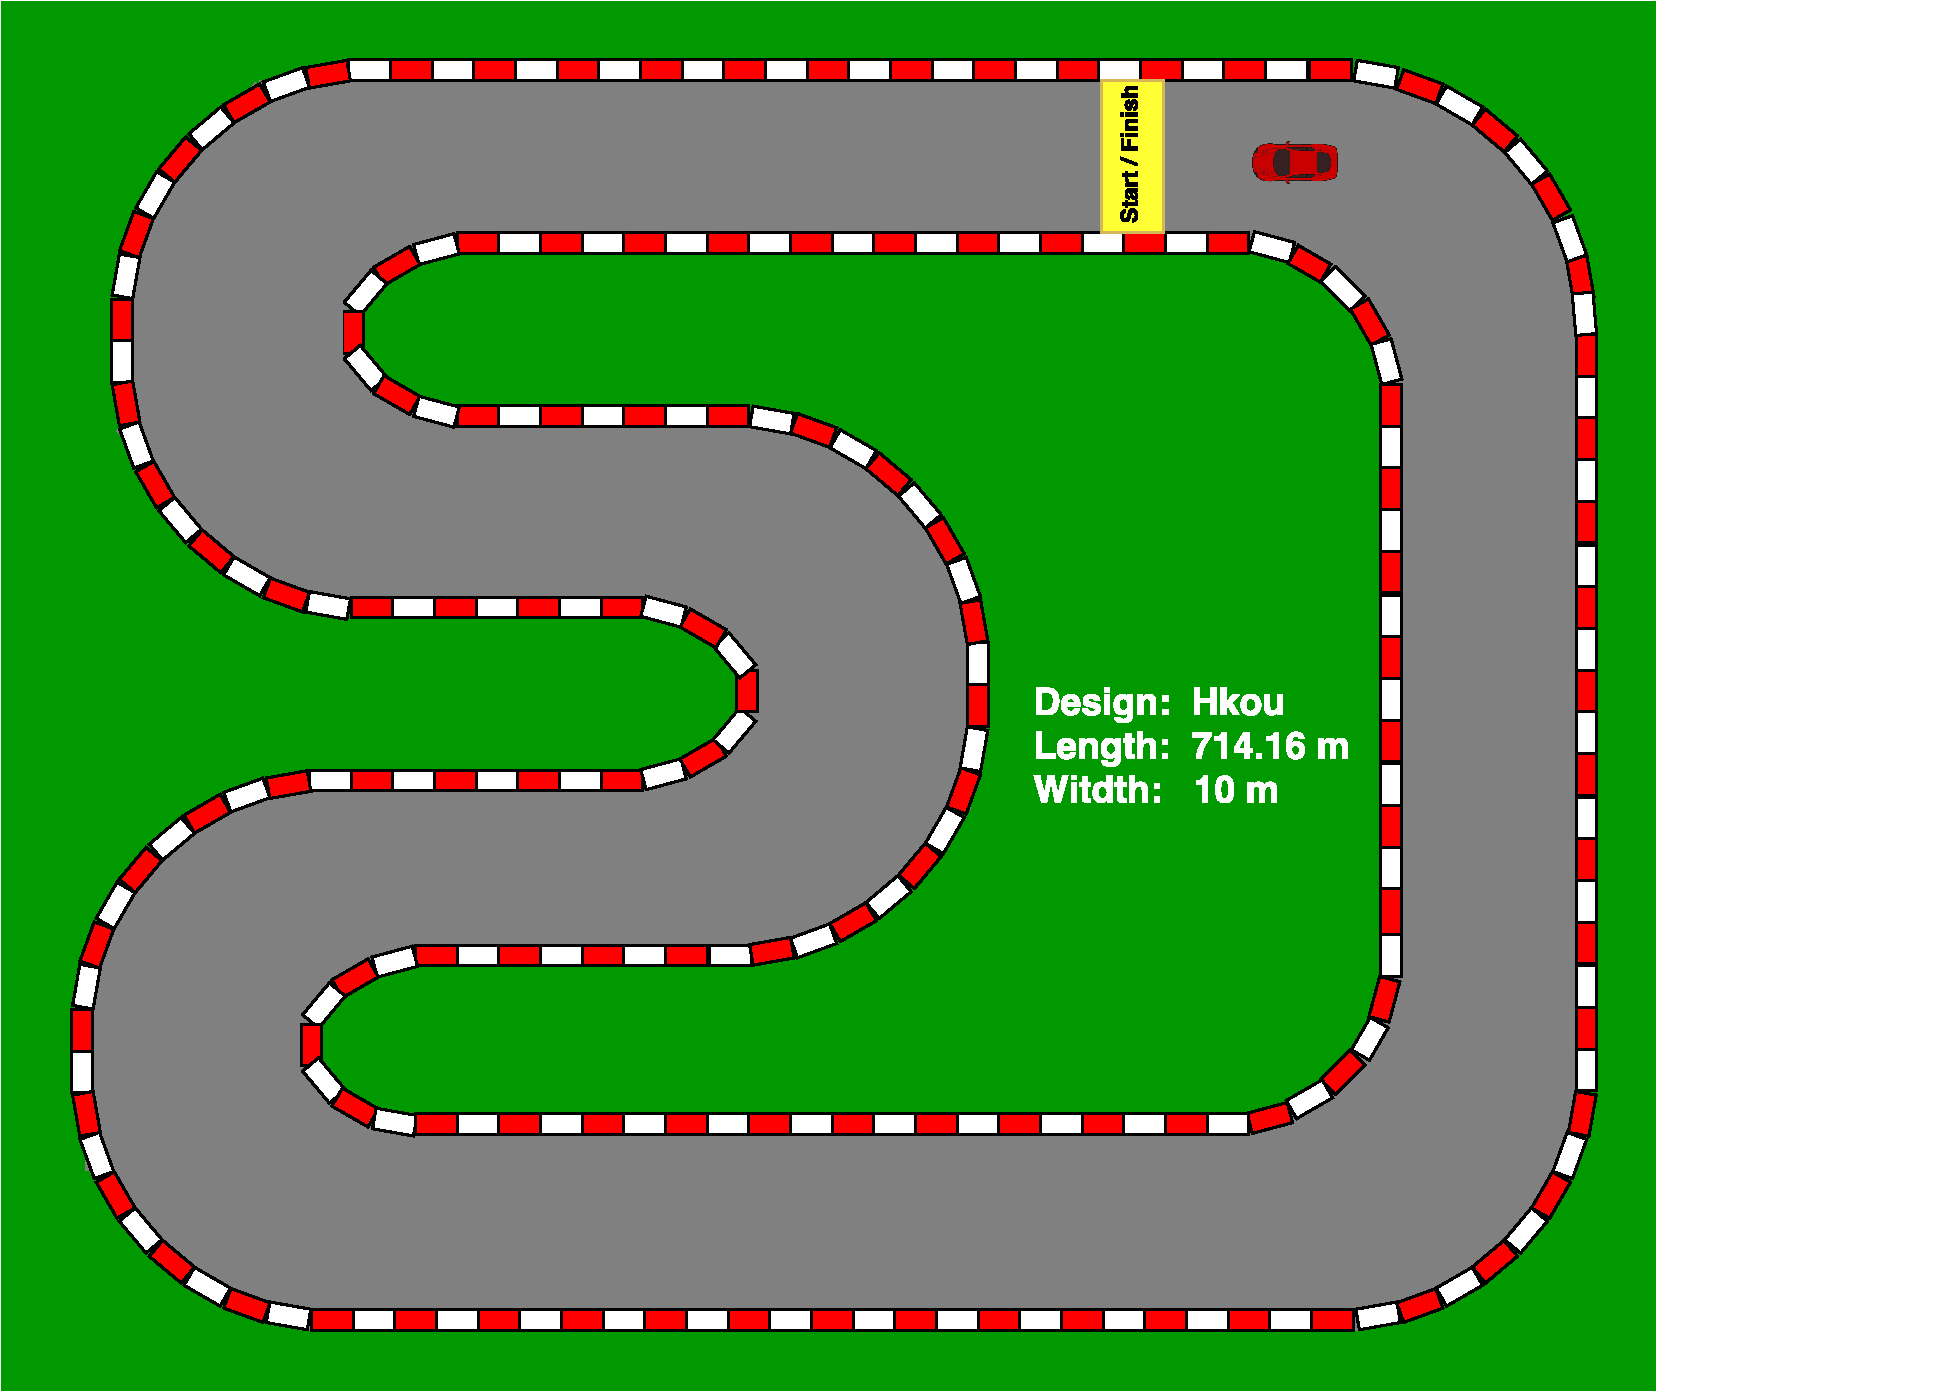
\includegraphics[width=1\textwidth]{Figures/Result/track_simple_2.pdf}
	\caption{The second track used is called $simple\_2$ made by Hkou}
	\label{fig:track_simple_2}
\end{figure}

The last track used in this project, also looks similar to the two other tracks on \Cref{fig:track_simple_1} and \Cref{fig:track_simple_2}. The track is simpler, it only has left turns. Another difference from the other two tracks is the length, it is much longer than the other tracks. The different length is used to test how the agent learns on a different track with a longer distance. The last track used in this project can be seen on \Cref{fig:track_longstr}.

\begin{figure}[H]
	\centering
	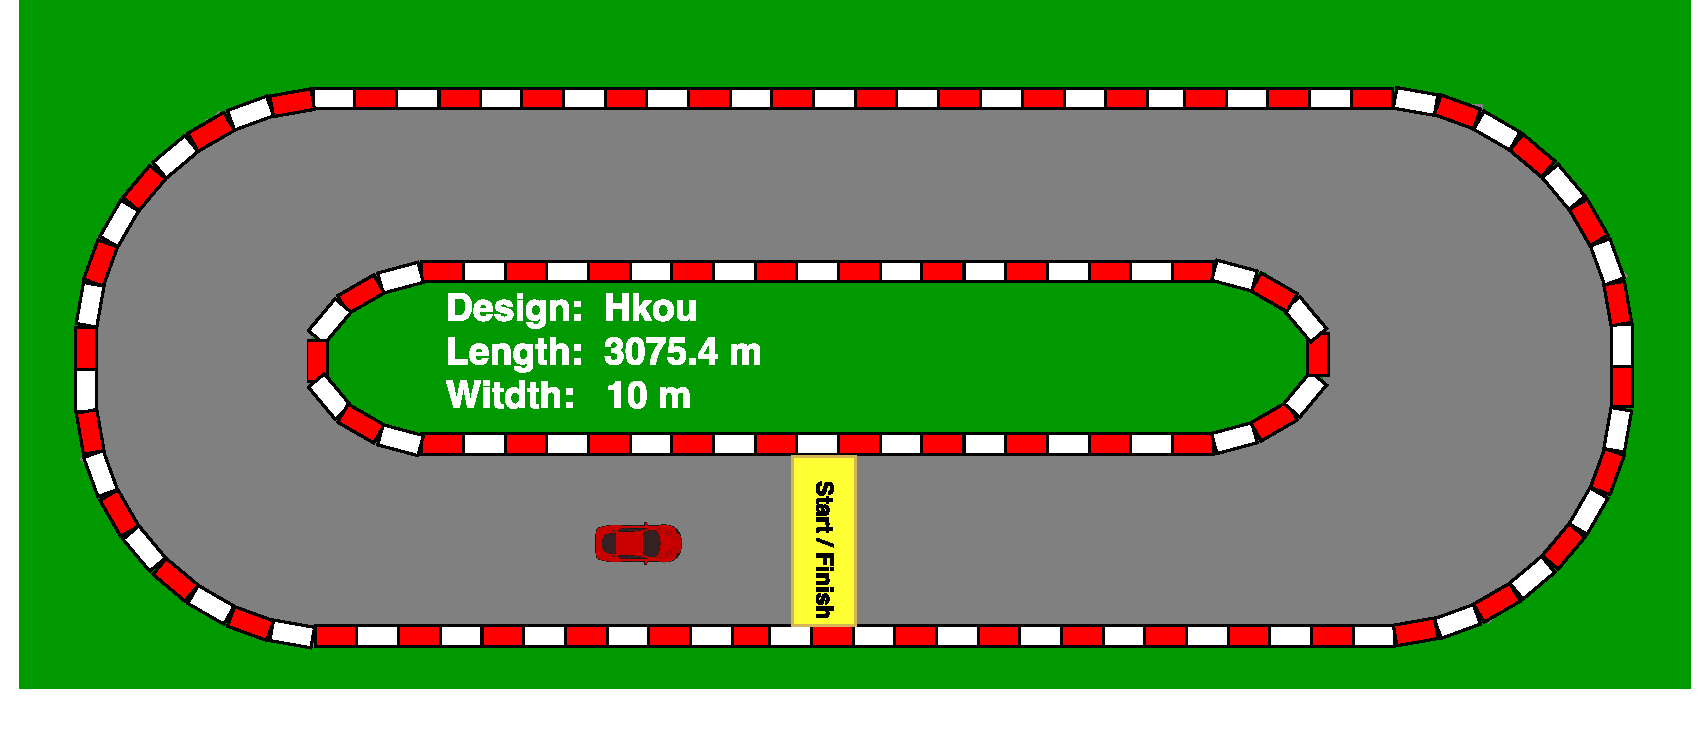
\includegraphics[width=1\textwidth]{Figures/Result/track_longstr.pdf}
	\caption{The third track used is called $longstr$ made by Hkou}
	\label{fig:track_longstr}
\end{figure}


\subsection*{Training}
It is tested if the tracks have an influence on the training. This is done to see if some of the used tracks are performing better on training than others. 

To compare the training, the reward graph is used. An agent with the same parameters, has trained on the three different tracks (\Cref{fig:track_simple_1}, \Cref{fig:track_simple_2} and \Cref{fig:track_longstr}). It is tested if the reward is growing faster on one of the tracks than the others, and even more important converge to the optimal reward faster. The reward graph can be seen on \Cref{fig:change_of_track_reward_graph}. 

\begin{figure}[H]
	\centering
	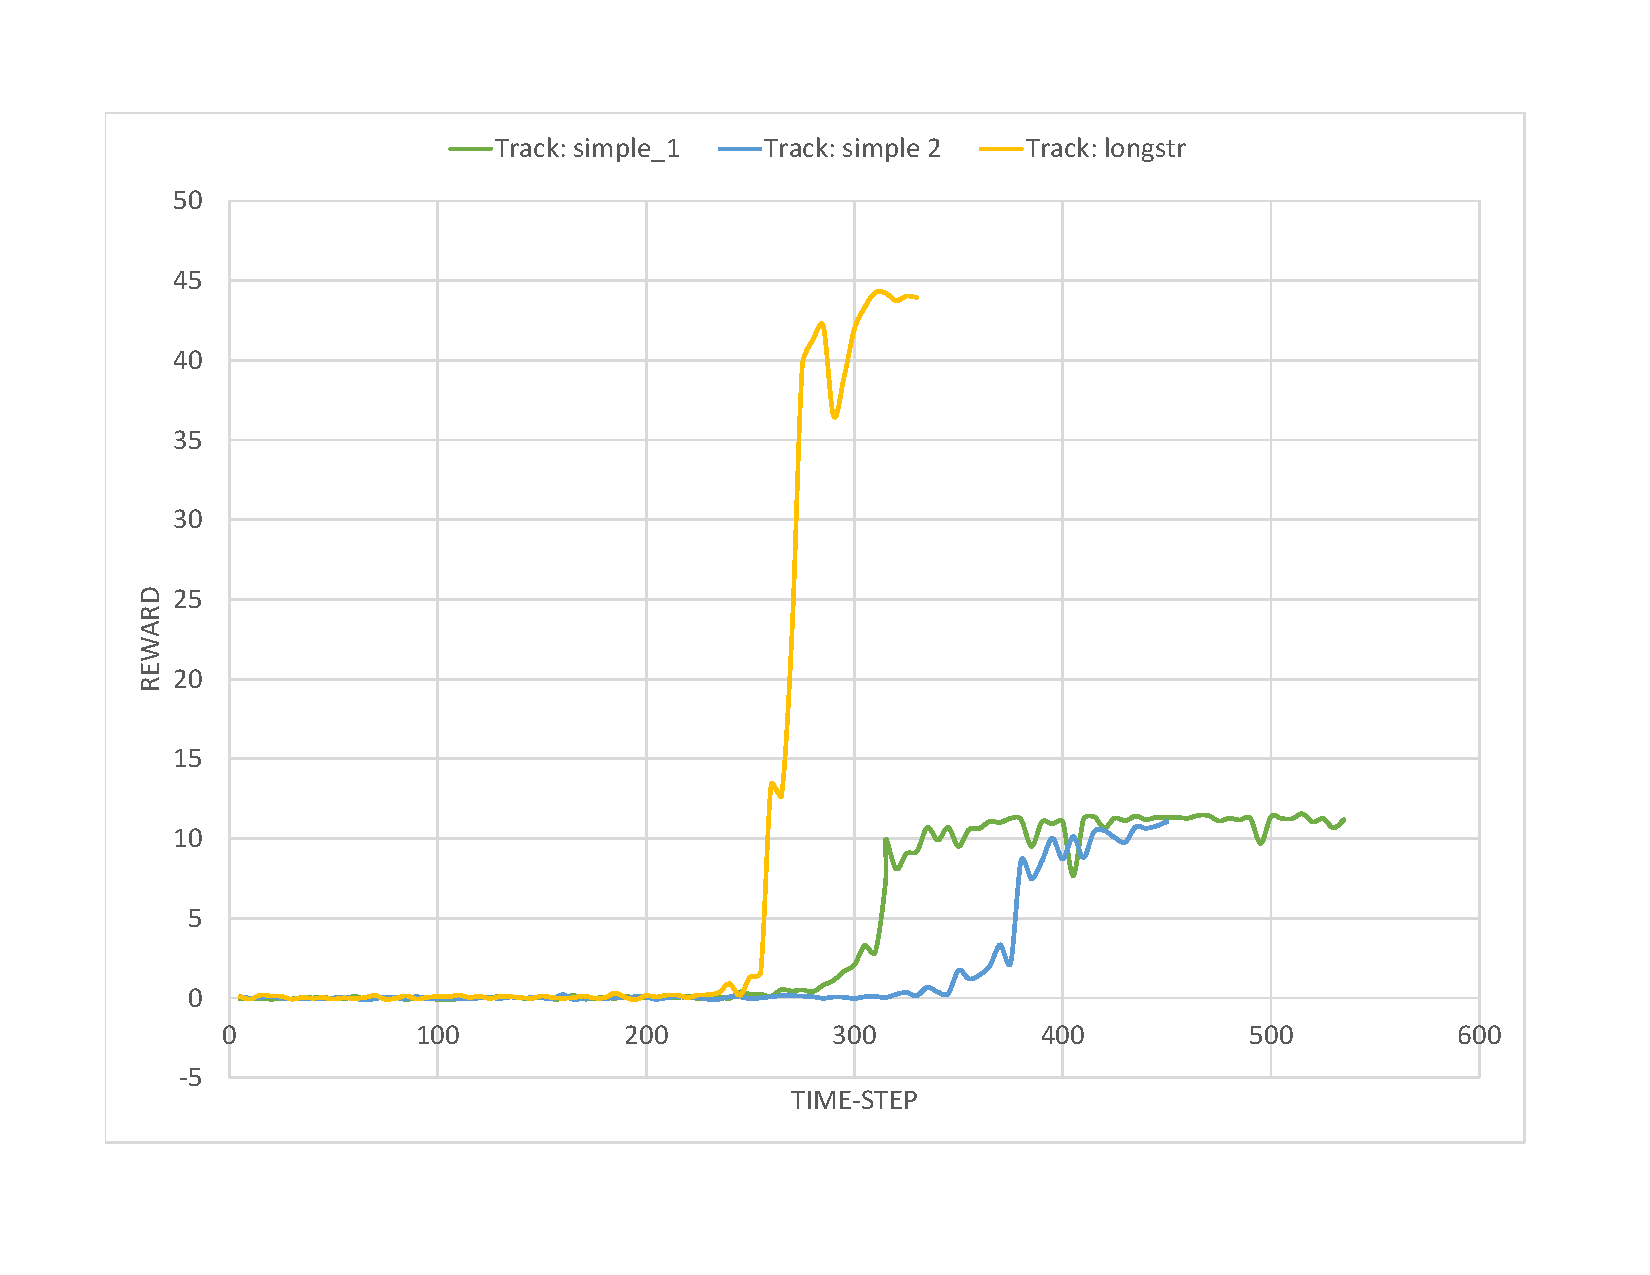
\includegraphics[width=1\textwidth]{Figures/Result/change_of_track_reward_graph.pdf}
	\caption{Comparison of the three different tracks with the reward getting from the environment}
	\label{fig:change_of_track_reward_graph}
\end{figure}

As seen on \Cref{fig:change_of_track_reward_graph} the different tracks has a small influence on when the reward starts learning. The track longstr learns around 250 time-steps, simple\_1 around 300 time-steps and simple\_2 around 350 time-steps. It is hard to say why the agent learns faster on the simple\_1 track than the simple\_2 track because it is the same track just mirrored. It could be the exploration on the simple\_1 track is better than the one on simple\_2. Here it also seems to learn the track longstr faster, this could be because it is a simpler track than the two other tracks.  

The biggest different on \Cref{fig:change_of_track_reward_graph} is the reward on the third track. This reward is converging to a bigger reward 44, than the reward from the two other tracks 11. This is due to the length of the track. Because the agent will get a bigger reward when the track is longer. The reward is given by every step and added together to a total reward, if there are more steps, then the total reward is bigger. Another way to look at it is the length of every time-step is longer. The length of the time-steps on the different tracks can be seen on \Cref{fig:change_of_track_length_graph}.     

\begin{figure}[H]
	\centering
	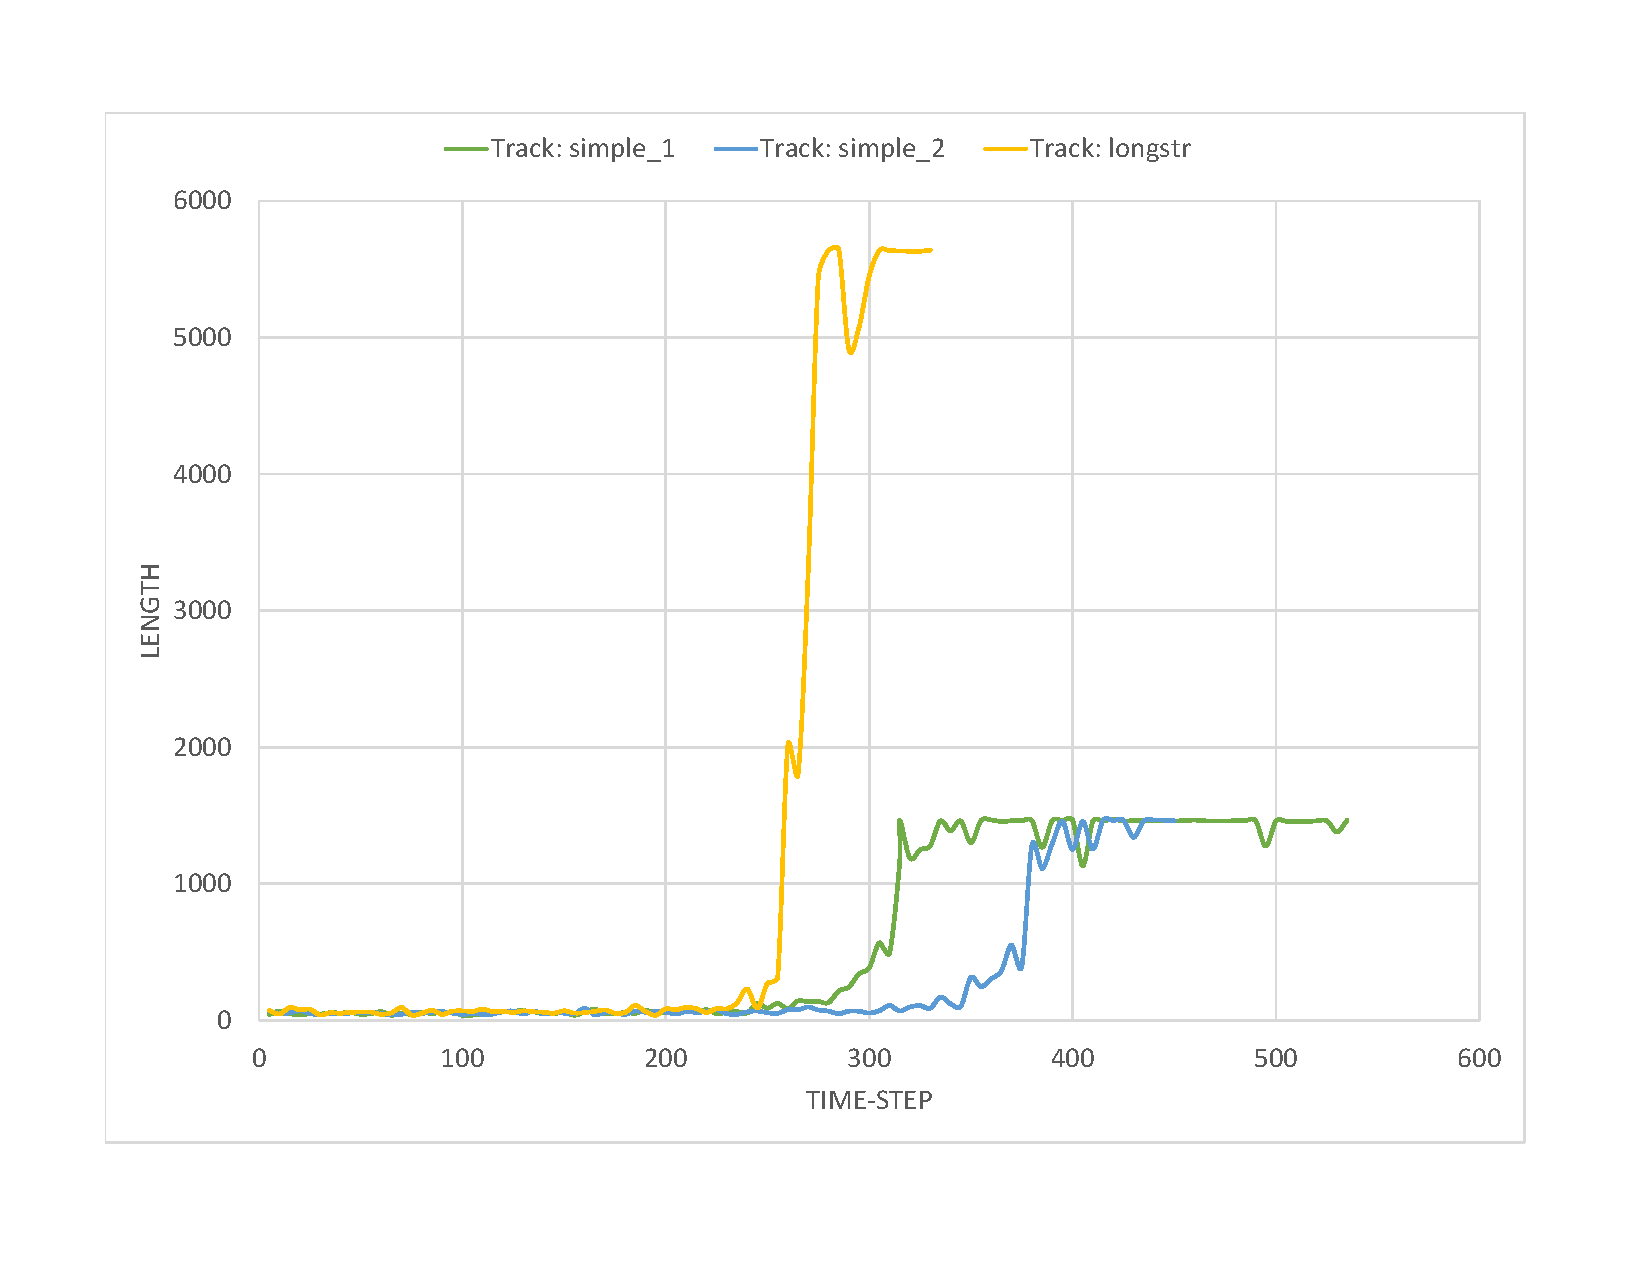
\includegraphics[width=1\textwidth]{Figures/Result/change_of_track_length_graph.pdf}
	\caption{Comparison of the three different tracks with the length of the episodes}
	\label{fig:change_of_track_length_graph}
\end{figure}

Because the track is 3-4 times longer the reward is also 3-4 times bigger:
\begin{equation}
\frac{\mathrm{Length \ of \ longstr}}{\mathrm{Length \ of \ simple\_1}} = \mathrm{Length \ difference}   \qquad \rightarrow \qquad \frac{3075.4}{714.16} = 4.31  
\end{equation}
\begin{equation}
\frac{\mathrm{Reward \ of \ longstr}}{\mathrm{Reward \ of \ simple\_1}} = \mathrm{Reward \ difference}   \qquad \rightarrow \qquad \frac{44}{11} = 4
\end{equation}
By looking at the result of the two equations, it looks like the bigger reward is the difference between the length of the tracks. 

After these result, the track which has been used in all the other training is the first track seen on \Cref{fig:track_simple_1}. To test if the agent has learned how to drive, the second track is used seen on \Cref{fig:track_simple_2}. If the agent can complete a lap on both tracks it is concluded the agent has learned how to drive.  
  



